\section{Experimental Results}
\label{sec:experimentalResults}
\subsection{Bootstrapping for Imagery with Noisy Labels}
\label{sec:results_bootstrapping}
The results from Experiment E1 and E2 comparing the bootstrapping methods and the baseline method at several levels of label noise, are displayed in Figure \ref{fig:E1_boot_mass} and Figure \ref{fig:E2_boot_norway}. The plots in the first figure shows the performance of models trained on patch examples from the Massachusetts Roads Dataset, whereas the second figure show results from training on patch examples from the Norwegian Roads Dataset. Experiment E2 also includes the performance of confident bootstrapping. \todo{og tabell til slutt. Ta ut caption og putt i tekst. Beskrive tabell bedre. Fjerne experimental design artifically added noise. Ikke resultat, nevn heller i setup. Være konsekvent i figurer. }\\

\begin{figure}
\begin{subfigure}{0.48\textwidth}
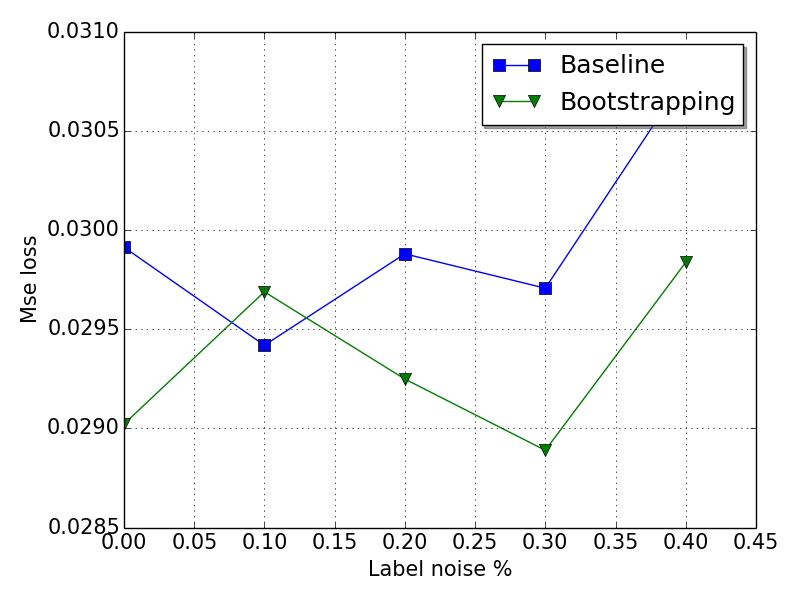
\includegraphics[width=\linewidth]{figs/E1/E1-lc-noise.png}
\caption{MSE test loss} \label{fig:E1_boot_mass_loss}
\end{subfigure}
\hspace*{\fill} % separation between the subfigures
\begin{subfigure}{0.48\textwidth}
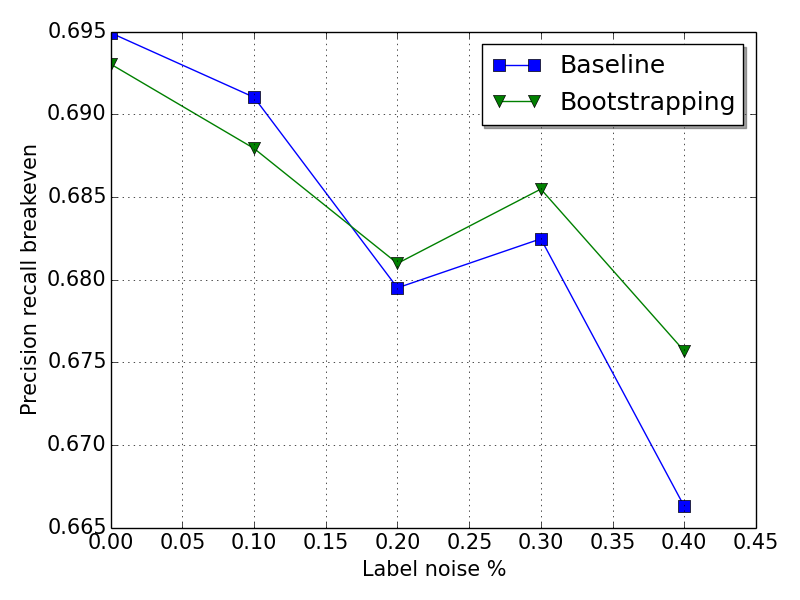
\includegraphics[width=\linewidth]{figs/E1/E1-pr-noise.png}
\caption{Precision and recall breakeven} \label{fig:E1_boot_mass_pr}
\end{subfigure}
\hspace*{\fill} % separation between the subfigures
\caption[E1 - Robustness of bootstrapping with  Massachusetts Roads Dataset]{E1 - Robustness of bootstrapping for increasing amount of label noise. Massachusetts Roads Dataset} \label{fig:E1_boot_mass}
\end{figure}

\begin{figure}
\begin{subfigure}{0.5\textwidth}
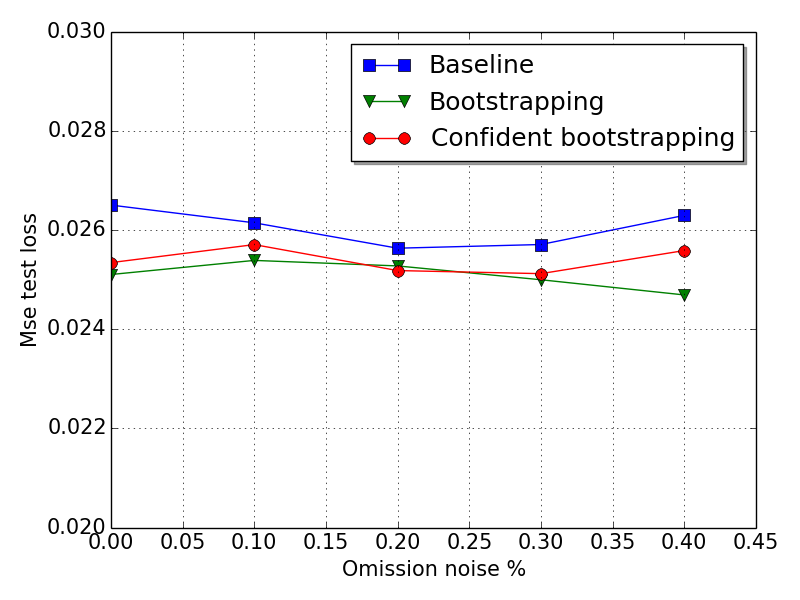
\includegraphics[width=\linewidth]{figs/E2/E2-lc-noise.png}
\caption{MSE test loss} \label{fig:E2_boot_norway_loss}
\end{subfigure}
\hspace*{\fill} % separation between the subfigures
\begin{subfigure}{0.5\textwidth}
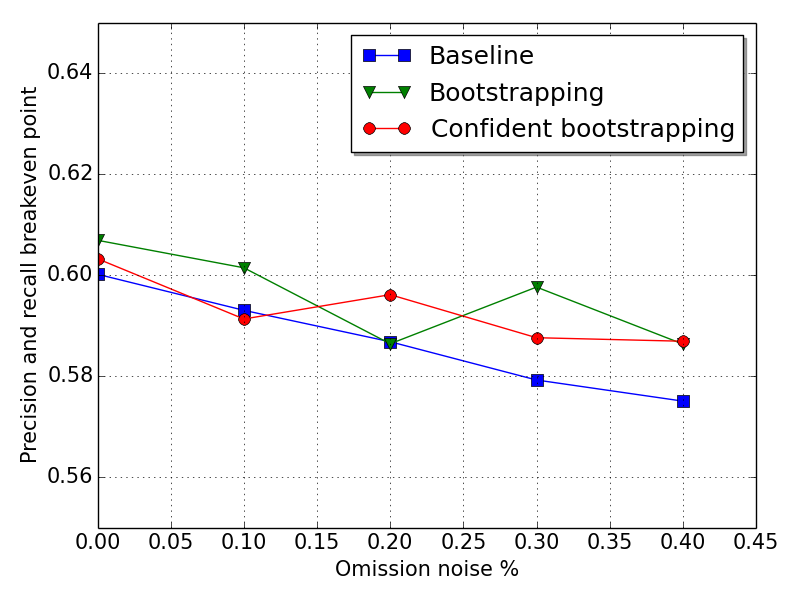
\includegraphics[width=\linewidth]{figs/E2/E2-pr-noise.png}
\caption{Precision and recall breakeven} \label{fig:E2_boot_norway_pr}
\end{subfigure}
\hspace*{\fill} % separation between the subfigures
\caption[E2 - Robustness of bootstrapping for increasing amount of label noise]{E2 - Robustness of bootstrapping for increasing amount of label noise. Norwegian Roads Dataset} \label{fig:E2_boot_norway}
\end{figure}

Figure \ref{fig:E1_boot_mass_loss} displays the test loss at different levels of label noise for Experiment E1. The baseline test loss, which utilizes the cross-entropy loss function, seems to generally increase as the noise level is increased. The bootstrapping loss function has a lower test loss compared to the baseline for noise levels above 10 percent.\\

Figure \ref{fig:E1_boot_mass_pr} displays the precision and recall breakeven points for increasing levels of label noise, and shows a trend of decreasing values.  At around 20 percent, the breakeven point of bootstrapping surpasses the baseline. However, the difference in performance seems to be small.\\

In Figure \ref{fig:E2_boot_norway_loss}, the test loss for bootstrapping and confident bootstrapping are consistently lower than the baseline. The test loss plots does not seem to increase as much as expected. Though, the precision and recall breakeven points of the baseline, decrease with increasing levels of omission noise. This can be seen in Figure \ref{fig:E2_boot_norway_pr}. Although the bootstrapping methods behave a bit more erratic, the plot seems to be decreasing at a slower rate. The plots also show that the overall difference in performance is small. Detailed figures of the precision and recall curves and test loss per epoch plots for each level of label noise can be found in Appendix \ref{app:fullE5results}. \\

A slightly different approach has been taken for Experiment E3. The road detection system has in this experiment been trained with labels from the label set N50, without adding artificial noise. The result from this experiment is displayed in Figure \ref{fig:E3_boot_norway_vbase}.\\

\begin{figure}
\begin{subfigure}{0.5\textwidth}
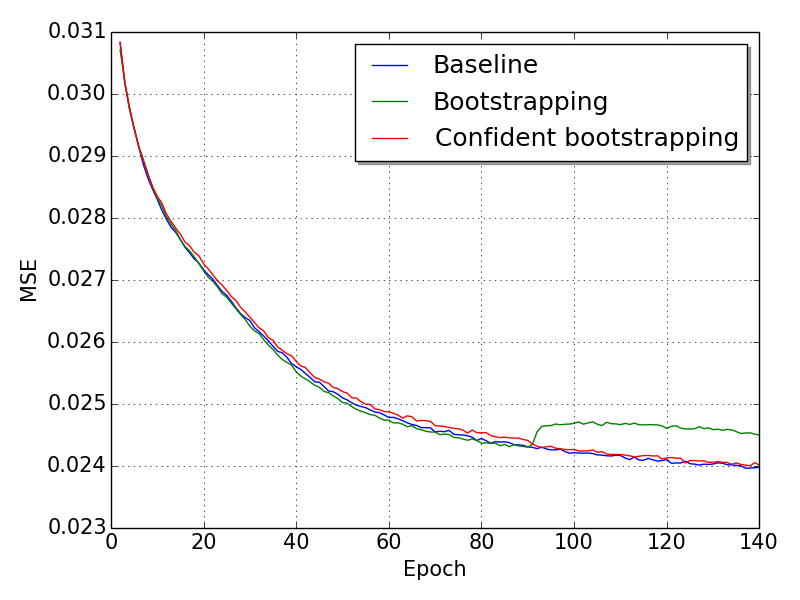
\includegraphics[width=\linewidth]{figs/E3/E3-lc.png}
\caption{MSE test loss} \label{fig:E3_boot_norway_vbase_loss}
\end{subfigure}
\hspace*{\fill} % separation between the subfigures
\begin{subfigure}{0.5\textwidth}
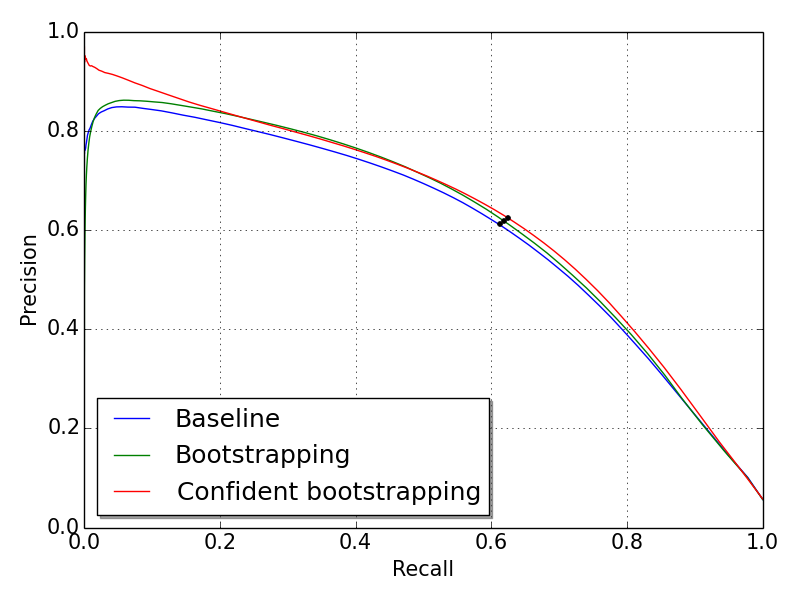
\includegraphics[width=\linewidth]{figs/E3/E3-pr.png}
\caption{Precision and recall comparison.} \label{fig:E3_boot_norway_vbase_pr}
\end{subfigure}
\hspace*{\fill} % separation between the subfigures
\caption[E3 - Comparison of loss functions for Norwegian Roads Dataset Vbase]{E3 - Comparison of loss functions for Norwegian Roads Dataset Vbase. The training set consists of labels with omission noise, and severe levels registration noise.} \label{fig:E3_boot_norway_vbase}
\end{figure}

The difference between bootstrapping and confident bootstrapping is evident in Figure \ref{fig:E3_boot_norway_vbase_loss}. After epoch 90, the factor $\beta$ is decreased in favour of the model predictions. The test loss of confident bootstrapping sees an immediate decrease compared to the baseline, whereas the bootstrapping test loss increase in value. In terms of test loss, the confident bootstrapping loss function performed comparably to the baseline loss function, while the regular bootstrapping loss function performed worse. However, this result is not evident from the precision and recall curve, displayed in Figure \ref{fig:E3_boot_norway_vbase_pr}. Both bootstrapping methods have better relaxed precision values  for every level of recall. \\

The results from Experiment E1, E2 and E3 are displayed in Table \ref{tab:results_bootstrapping_breakeven}. The table contains a row for every test, which includes  the percentage of artificial omission noise, precision and recall breakeven point, test loss and a p-value. The p-values are computed by the Welch's t-test from test loss samples of two different methods. For instance, the p-value of {\it E1 - bootstrapping 0\%} are computed by the test loss samples of {\it E1 - Bootstrapping 0\%} and {\it E1 - Baseline 0\%}.  If a p-value is below the significance level of 0.1, it is plausible that the samples originate from a distribution different from the distribution of the baseline samples. For the most part, the bootstrapping results are not statistically significant\todo{Need to check this}.\\



\begin{table}
\caption[Bootstrapping results]{Bootstrapping results.}
 \vspace{-0.65cm}
\begin{center}
\begin{adjustbox}{max width=\textwidth}
\begin{tabular}{+l ^l ^l ^r ^r ^r}\hline
\rowstyle{\bfseries}
  Experiment & \% & Dataset & Breakeven & Test loss & P-value\\\hline
  E1 - Baseline 			&0	& Massachusetts & 0.6949 & 0.0299 & - \\
  E1 - Baseline 			&10 & Massachusetts & 0.6910 & 0.0294 & -  \\
  E1 - Baseline 			&20 & Massachusetts & 0.6795 & 0.0299 & - \\
  E1 - Baseline 			&30 & Massachusetts & 0.6825 & 0.0297 & - \\
  E1 - Baseline 			&40 & Massachusetts & 0.6663 & 0.0308 & - \\
  E1 - Bootstrapping 	&0	& Massachusetts & 0.6930 & 0.0290 & 0.15164 \\
  E1 - Bootstrapping 	&10 & Massachusetts & 0.6879 & 0.0297 & 0.64355  \\
  E1 - Bootstrapping 	&20 & Massachusetts & 0.6810 & 0.0292 & 0.25650 \\
  E1 - Bootstrapping 	&30 & Massachusetts & 0.6855 & 0.0289 & 0.22492 \\
  E1 - Bootstrapping 	&40 & Massachusetts & 0.6757 & 0.0299 & 0.15764 \\\hline
  E2 - Baseline 			&0	& Norwegian & 0.6001 & 0.0265 & - \\
  E2 - Baseline 			&10 	& Norwegian & 0.5930 & 0.0261 & -  \\
  E2 - Baseline 			&20 	& Norwegian & 0.5868 & 0.0256 & - \\
  E2 - Baseline 			&30 	& Norwegian & 0.5792 & 0.0257 & - \\
  E2 - Baseline 			&40 	& Norwegian & 0.5750 & 0.0263 & - \\
  E2 - Bootstrapping 	&0	& Norwegian & 0.6069 & 0.0251 & 0.09136 \\
  E2 - Bootstrapping 	&10 & Norwegian & 0.6014 & 0.0254 & 0.29272 \\
  E2 - Bootstrapping 	&20 & Norwegian & 0.5864 & 0.0252 & 0.48285 \\
  E2 - Bootstrapping 	&30 & Norwegian & 0.5976 & 0.0250 & 0.11260 \\
  E2 - Bootstrapping 	&40 & Norwegian & 0.5863 & 0.0247 & 0.00480 \\
  E2 - Confident 		&0	& Norwegian & 0.6032 & 0.0253 & 0.09433 \\
  E2 - Confident 		&10 & Norwegian & 0.5913 & 0.0257 & 0.43790 \\
  E2 - Confident 		&20 & Norwegian & 0.5961 & 0.0252 & 0.36447 \\
  E2 - Confident 		&30 & Norwegian & 0.5876 & 0.0251 & 0.09397 \\
  E2 - Confident 		&40 & Norwegian & 0.5869 & 0.0256 & 0.17952 \\\hline
  E3 - Baseline 			&0 & Norwegian &  0.6114 & 0.0240 & - \\
  E3 - Bootstrapping 	&0 & Norwegian &  0.6186 & 0.0245 & 0.18114 \\
  E3 - Confident 		&0 & Norwegian &  0.6244 & 0.0240 & 0.90851  \\
  \hline
\end{tabular}
\end{adjustbox}
\end{center}
\label{tab:results_bootstrapping_breakeven}
\end{table}

\subsection{Curriculum Learning with Aerial Imagery}
\label{sec:results_curriculum_learning_aerial_imagery}
Curriculum learning was tested in Experiment E4, E5 and E6. Results from Experiment E4 are displayed in Table \ref{fig:E4_curriculum_mass}, whereas results from Experiment E5 are displayed in Table \ref{fig:E5_curriculum_norway}. In addition, Experiment E4 explores anti-curriculum learning, while Experiment E5 tests patch datasets constructed with various difficulty thresholds $D_0$. Finally, Experiment E6 investigates gradual curriculum learning and the performance of only training with the first stage of a curriculum patch dataset.\\

Experiment E4 was conducted using the Massachusetts Roads Dataset. In Figure \ref{fig:E4_curr_mass_loss}, the switch from stage 0 to stage 1 at epoch 50 is clearly visible for the \textit{curriculum} and \textit{anti-curriculum} test loss plots. The network trained with the curriculum patch dataset, performed better than the baseline as seen in Figure \ref{fig:E4_curr_mass_loss} and Figure \ref{fig:E4_curr_mass_pr}. The test loss gap between the \textit{baseline} and \textit{curriculum} is largest before epoch 50, but is still maintained to a lesser extent after. The precision and recall breakeven point of \textit{curriculum} is above that of the \textit{baseline} as well.   \\

\begin{figure}
\begin{subfigure}{0.5\textwidth}
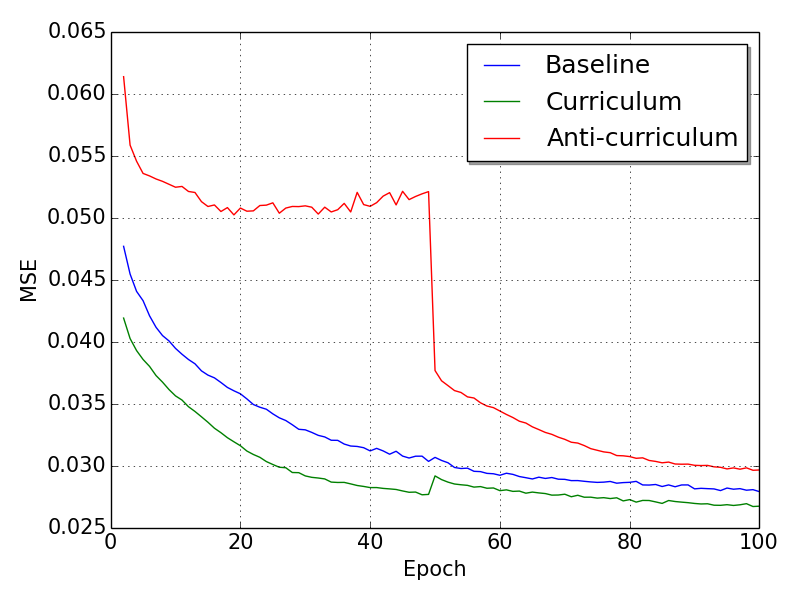
\includegraphics[width=\linewidth]{figs/E4/E4-lc.png}
\caption{Comparison of test loss} \label{fig:E4_curr_mass_loss}
\end{subfigure}
\hspace*{\fill} % separation between the subfigures
\begin{subfigure}{0.5\textwidth}
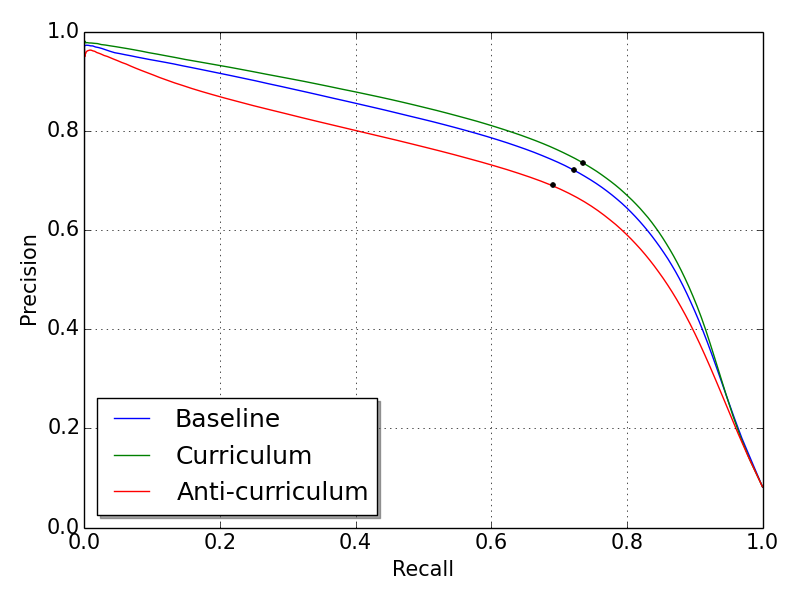
\includegraphics[width=\linewidth]{figs/E4/E4-pr.png}
\caption{Precision and recall comparisons.} \label{fig:E4_curr_mass_pr}
\end{subfigure}
\hspace*{\fill} % separation between the subfigures
\caption[E4 - Performance of curriculum learning for Massachusetts Roads Dataset]{E4 - Performance of curriculum learning and anti-curriculum learning for Massachusetts Roads Dataset} \label{fig:E4_curriculum_mass}
\end{figure}

Training with an anti-curriculum strategy, where the first stage consists of harder examples, seemed to do worse than both the \textit{baseline} and \textit{curriculum}. This is especially evident in the test loss plot, where the the test loss stagnates at around epoch 25, and starts to overfit towards epoch 50. From epoch 50 when stage 1 examples entered the training set, there is a dramatic decrease in test loss. The test loss decrease continues at a steady pace until epoch 85. Yet, the final performance of anti-curriculum learning is substantially lower than both the baseline and curriculum learning, as illustrated by the breakeven points in Figure \ref{fig:E4_curr_mass_pr}.\\

The training set difficulty distribution, according to the difficulty estimator $d(y,q)$ from Experiment E4, is illustrated in a histogram in Figure \ref{fig:E4_difficulty_distribution}. The training set of  Massachusetts Roads Dataset was sampled, and the difficulty estimate for each patch was computed for every patch. Patches that contained no road label pixels, were counted separately from patches that contained road label pixels. The resulting histogram for non-road patches in Figure \ref{fig:E4_difficulty_distribution_nonroad}, shows that the trained curriculum teacher of Experiment E4 is excellent at predicting non-road patches, because the predictions and labels match very well. This results in very low difficulty estimates. This is not the case for road patches, illustrated by Figure  \ref{fig:E4_difficulty_distribution_road}, where the distribution is clearly skewed right and have a greater variance. \\

\begin{figure}
\begin{subfigure}{0.5\textwidth}
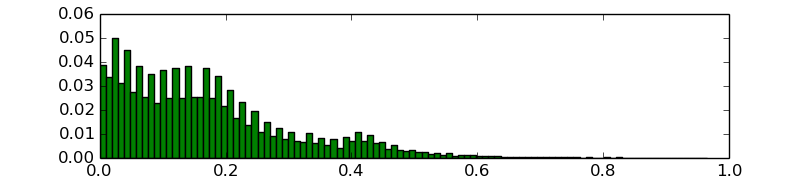
\includegraphics[width=\linewidth]{figs/E4/E4-road-dist.png}
\caption{Distribution for road patches.} \label{fig:E4_difficulty_distribution_road}
\end{subfigure}
\hspace*{\fill} % separation between the subfigures
\begin{subfigure}{0.5\textwidth}
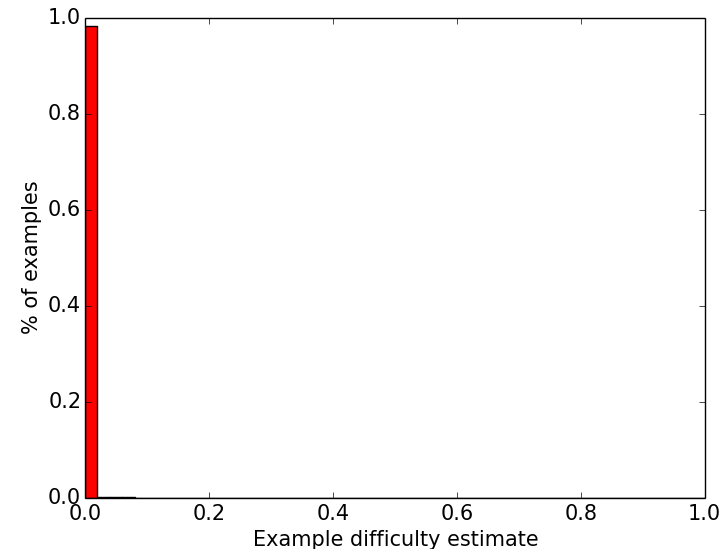
\includegraphics[width=\linewidth]{figs/E4/E4-non_road-dist.png}
\caption{Distribution for non-road patches.} \label{fig:E4_difficulty_distribution_nonroad}
\end{subfigure}
\hspace*{\fill} % separation between the subfigures
\caption[E4 - Difficulty distribution]{E4 - Example difficulty distribution according to estimator $d(y,q)$. } \label{fig:E4_difficulty_distribution}
\end{figure}

In Experiment E5, the road detection system was trained on four different patch datasets created from the Norwegian Roads Dataset. A comparison of the test loss per epoch is displayed in Figure \ref{fig:E5_curr_norway_loss}, whereas the final performance of each patch dataset is shown by a precision and recall curve in Figure \ref{fig:E5_curr_norway_pr}. The network configuration used for the tests was identical, as well as the number of training examples seen during training. Essentially, the gap between the \textit{baseline} and \textit{curriculum} curves, comes from the first stage of the patch datasets, where different difficulty threshold $D_0$ have been used.\\

\begin{figure}[h]
\begin{subfigure}{0.5\textwidth}
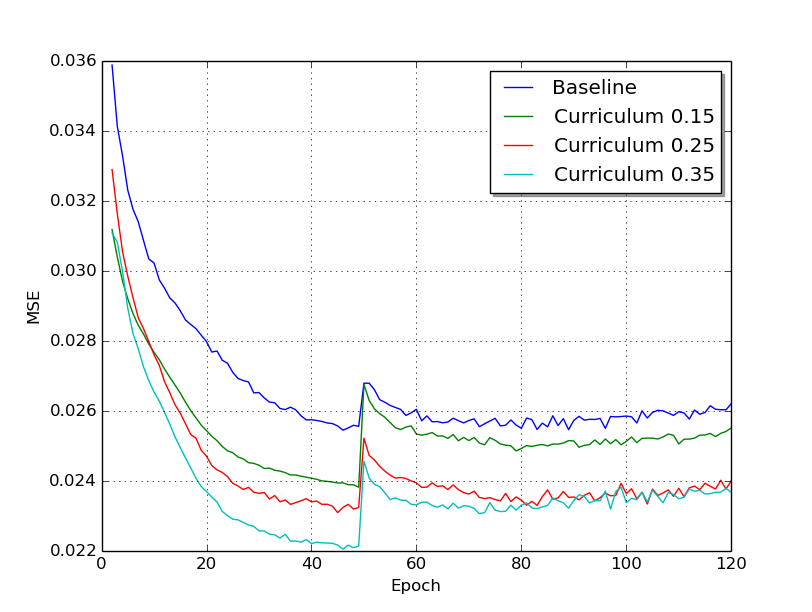
\includegraphics[width=\linewidth]{figs/E5/E5-lc.png}
\caption{Comparison of test loss} \label{fig:E5_curr_norway_loss}
\end{subfigure}
\hspace*{\fill} % separation between the subfigures
\begin{subfigure}{0.5\textwidth}
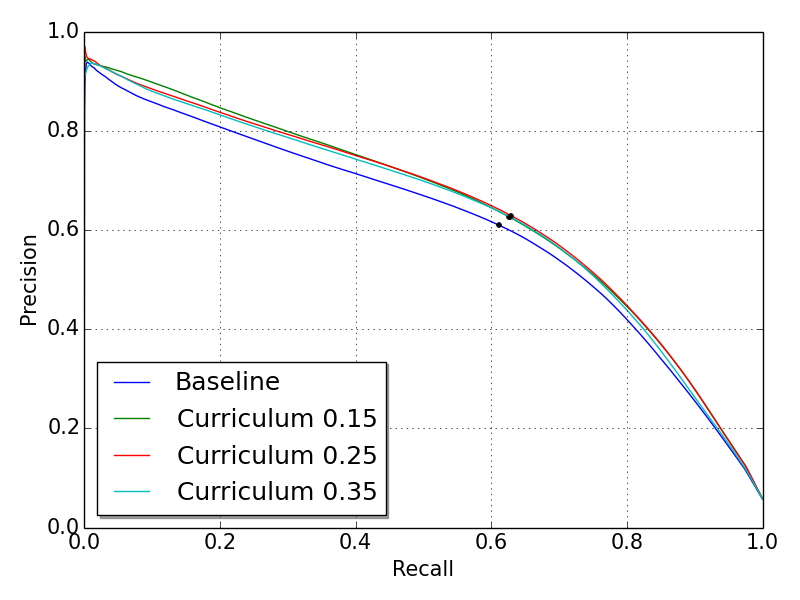
\includegraphics[width=\linewidth]{figs/E5/E5-pr.png}
\caption{Precision and recall comparisons.} \label{fig:E5_curr_norway_pr}
\end{subfigure}
\hspace*{\fill} % separation between the subfigures
\caption[E5 - Performance of curriculum learning for Norwegian Roads Dataset Vbase]{E5 - Performance of curriculum learning at different thresholds, $D_{0}$ for Norwegian Roads Dataset Vbase} \label{fig:E5_curriculum_norway}
\end{figure}

Observing the plots in Figure \ref{fig:E5_curr_norway_loss}, the switch from stage 0 to stage 1, is clearly visible at epoch 50. The increase in test loss is most severe in the datasets formed by a curriculum strategy. Leading up to epoch 50, the curriculum plots show an increasing gap in test performance, if compared to the baseline plot. After the switch the curriculum datasets still outperform the baseline dataset, even though the example distribution of stage 1 are the same for all patch datasets.\\

In Figure \ref{fig:E5_curr_norway_pr}, the networks trained with a curriculum strategy shows an improved relaxed precision for all levels of recall compared to the baseline.\\

An interesting trend between the thresholds $D_0$ and the loss, is that decreasing the difficulty threshold, does not necessarily produce better results. The patch dataset \textit{Curriculum 0.15} has the easiest first stage, yet performed worse than \textit{Curriculum 0.25} and \textit{Curriculum 0.35}.\\

Figure \ref{fig:E6_curriculum_inexperienced} shows the results from Experiment E6. The patch datasets in this experiment were created from a teacher that was trained with the same number of training examples as the patch datasets. Curriculum learning still achieved a higher test loss and gave better relaxed precision for all levels of releaxed recall, compared to the baseline.\\

Figure \ref{fig:E6_curriculum_inexperienced_loss} and \ref{fig:E6_curriculum_inexperienced_pr} illustrate the performance of training with only the first stage of the patch datasets. As expected, the first stage baseline has a lower breakeven point than the two stage baseline. More surprisingly, the first stage curriculum outperformed both the baseline and the curriculum, both in terms of breakeven point and test loss. However, at recall levels less than 0.4, the precision of the first stage curriculum decreases rapidly. \\

%This shows that the curriculum strategy is effective at filtering out inconsistent labels, and with a suitable difficulty threshold $D_0$ can provides enough example variability in the first stage training set. Another possible reason for this result, is the sudden training set switch at epoch 60, which dramatically increases the test loss. \\

\begin{figure}
\begin{subfigure}{0.5\textwidth}
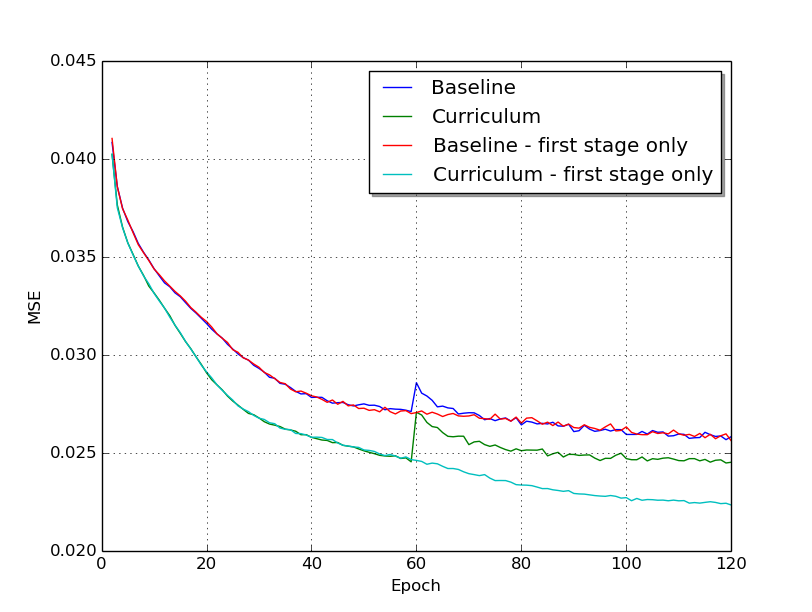
\includegraphics[width=\linewidth]{figs/E6/E6_lc_two_stage.png}

\caption{Test loss for two stage dataset}
\vspace{0.4cm} 
\label{fig:E6_curriculum_inexperienced_loss}
\end{subfigure}
\hspace*{\fill} % separation between the subfigures
\begin{subfigure}{0.5\textwidth}
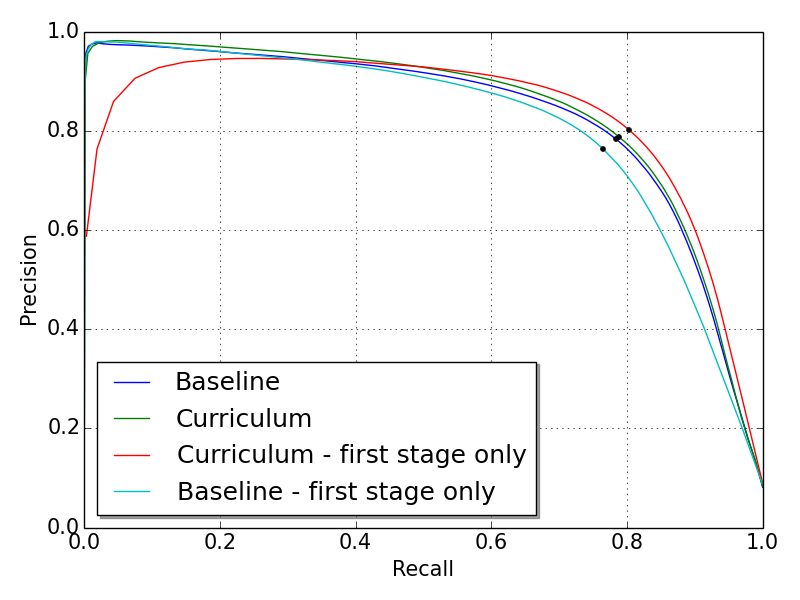
\includegraphics[width=\linewidth]{figs/E6/E6_pr_two_stage.png}
\caption{Precision and recall comparisons for two stage dataset.} \label{fig:E6_curriculum_inexperienced_pr}
\end{subfigure}

\begin{subfigure}{0.5\textwidth}
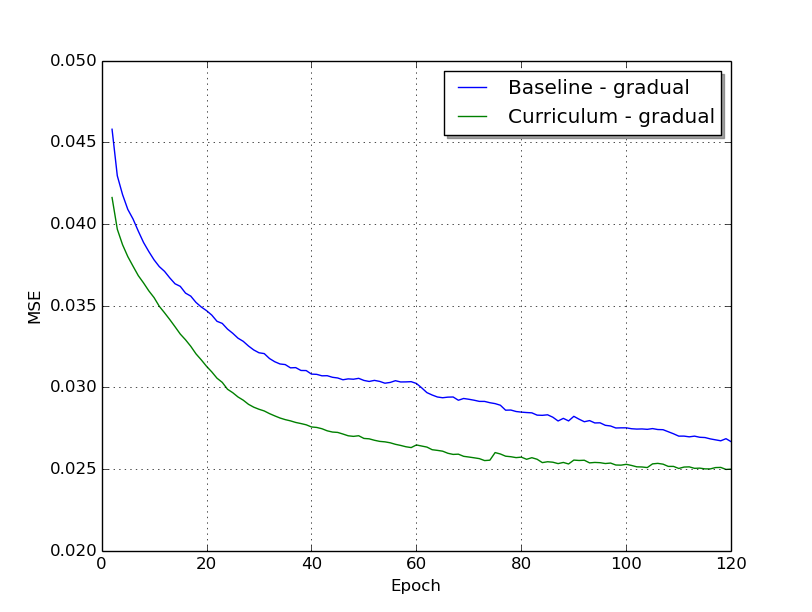
\includegraphics[width=\linewidth]{figs/E6/E6_lc_gradual.png}
\caption{Test loss for dataset with gradual stage switching} \label{fig:E6_gradual_loss}
\end{subfigure}
\hspace*{\fill} % separation between the subfigures
\begin{subfigure}{0.5\textwidth}
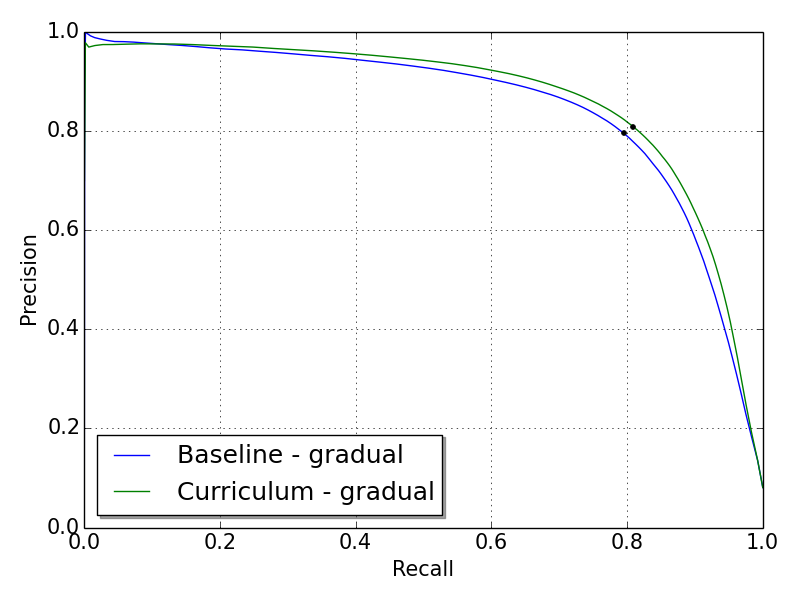
\includegraphics[width=\linewidth]{figs/E6/E6_pr_gradual.png}
\caption{Precision and recall for dataset with gradual stage switching.} \label{fig:E6_gradual_pr}
\end{subfigure}
\hspace*{\fill} % separation between the subfigures
\caption[E6 - Results from experiments with an less experienced teacher ]{E6 - Results from experiments with an less experienced teacher model.} \label{fig:E6_curriculum_inexperienced}
\end{figure}

This was further explored by creating two additional patch datasets, with 5 stages each. The first stage has 108000 examples, while the other 4 stages contain 54000 examples each. Subsequent stages replaces the training set, by assigning each example to a random position in the training set. Because the positions are picked by random sampling with replacement, only around 40\% of the existing examples in the training set are replaced at each switch. This results in a more gradual transition of the difficulty distribution. In Figure \ref{fig:E6_gradual_loss}, the stage switching with these patch datasets, results in the test loss being more stable.
The baseline plot even decreases substantially after epoch 60. This is an improvement from the spiking behaviour from the two stage baseline. The gradual approach also shows promise in Figure \ref{fig:E6_curriculum_inexperienced}, where the curriculum plot achieves a breakeven point of 0.809, compared to the breakeven of 0.802 for the first stage curriculum. The gradual baseline approach only achieved a breakeven of 0.795.\\



The precision and recall breakeven values from Experiment E4 and Experiment E5, are listed in Table \ref{tab:results_curriculum_learning_breakeven}, and shows that training with a curriculum strategy was beneficial for both datasets.\\


\begin{table}
\caption[Curriculum learning results]{Curriculum learning results. P-values are computed for the test loss. The Welch's t test compare the experiment and baseline distribution. If a p-value is below 0.1, it is plausible that the samples originate from different distributions.}
\begin{center}
\begin{adjustbox}{max width=\textwidth}
\begin{tabular}{+p{3.3cm} ^l ^l ^r ^r ^r}\hline
\rowstyle{\bfseries}
  Experiment & $\mathbf{D_0}$ & Dataset & Breakeven & Test loss & P-value\\\hline
  E4 - Baseline 		&1.0& Massachusetts & 0.7211 & 0.0279 & - \\
  E4 - Curriculum 	&0.25& Massachusetts & \textbf{0.7353} & 0.0267 & 0.01023 \\
  E4 - Anti-curriculum &0.25 & Massachusetts & 0.6904 & 0.0296 & 0.00057 \\\hline
  E5 - Baseline 		& 1.00 & Norwegian & 0.6105 & 0.0262 & -  \\
  E5 - Curriculum 	&0.15 & Norwegian & 0.6264 & 0.0255 & 0.18160 \\
  E5 - Curriculum 	&0.25 & Norwegian & \textbf{0.6292} & 0.0240 & 0.00817 \\
  E5 - Curriculum 	&0.35 & Norwegian & 0.6269 & 0.0237 & 0.00017 \\\hline
  E6 - Baseline 		&1.00 & Massachusetts & 0.7836 & 0.0258 & - \\
  E6 - Curriculum 	&0.25 & Massachusetts & 0.7880 & 0.0245 & 0.01519 \\
  E6 - Baseline, gradual 	&1.00 & Massachusetts & 0.7952 			&0.0267 & - \\
  E6 - Curriculum, gradual 	&0.25 & Massachusetts & \textbf{0.8088} 	&0.0250 & 0.00007 \\
  \hline
\end{tabular}
\end{adjustbox}
\end{center}
\label{tab:results_curriculum_learning_breakeven}
\end{table}

\subsection{Road Detection System}
\label{sec:results_road_detection_system}
In Experiment E7, the road detection system was trained on a much larger patch dataset than in previous sections. In order for the patch dataset to fit in main memory, the examples were split into nine separate stages each containing 442800 training examples. The content of the training set was switched during training. These switches are noticeable in the training loss plot in Figure \ref{fig:E7_performance_mass_lc}, where the loss increases slightly after a training set switch. The network converged to a \ac{MSE} test loss of 0.0232. \\

In Figure \ref{fig:E7_performance_mass_pr}, the averaged precision and recall curve is displayed. The precision and recall breakeven point for the system is 0.8341. Comparable experiments conducted in other works, are listed in Table \ref{tab:results_curriculum_learning_breakeven}. These systems have been described in Section \ref{sec:related_works}.\\

\begin{figure}
\begin{subfigure}{0.5\textwidth}
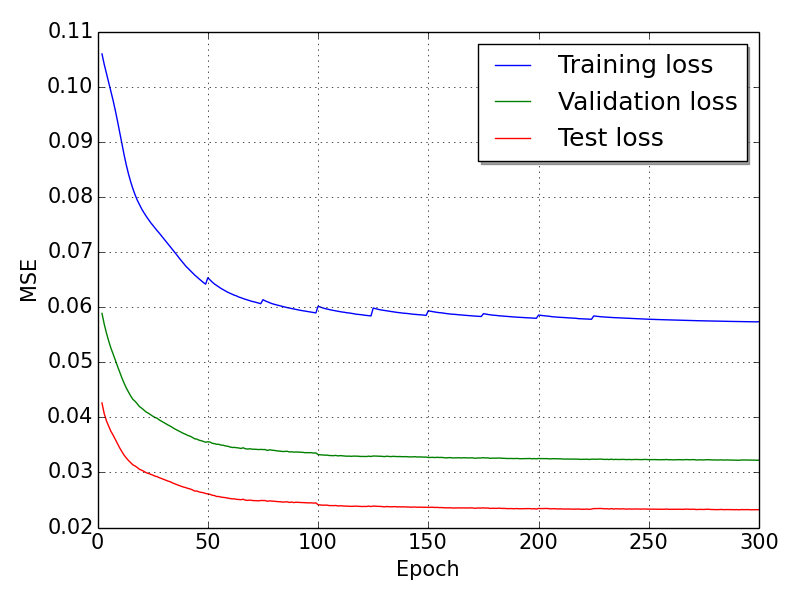
\includegraphics[width=\linewidth]{figs/E7/E7_lc_loss.png}
\caption{MSE loss} \label{fig:E7_performance_mass_lc}
\end{subfigure}
\hspace*{\fill} % separation between the subfigures
\begin{subfigure}{0.5\textwidth}
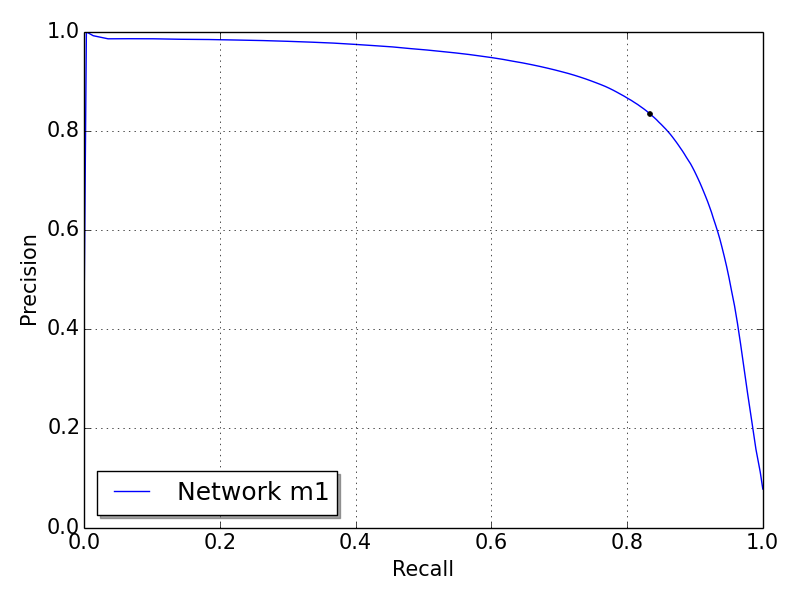
\includegraphics[width=\linewidth]{figs/E7/E7_pr.png}
\caption{Precision and recall.} \label{fig:E7_performance_mass_pr}
\end{subfigure}
\hspace*{\fill} % separation between the subfigures
\caption[E7 - Performance of the M1 road detection system trained with Massachusetts Roads Dataset]{E7 - Performance of the M1 road detection system trained with Massachusetts Roads Dataset.} \label{fig:E7_performance_mass}
\end{figure}

\begin{table}[H]
\caption[Road detection system results]{Road detection system results. The values in this table represent the precision and recall breakeven points achieved by the systems.}
\centering
\begin{tabular}{+l ^r ^r}\hline
\rowstyle{\bfseries}
  System & breakeven & best network\\\hline
  M1 - Network & 0.8341 & 0.8413\\
  M2 - Network & 0.8494 & 0.8627\\
  \cite{MnihThesis}\tablefootnote{The number of experiment runs is unclear.} & 0.8873 & \\
  \cite{saito_building_and_roads}\tablefootnote{See footnote 1.} & 0.8866& \\\hline
  N1 - Network & 0.7508 & 0.7620 \\\hline
\end{tabular}
\label{tab:results_curriculum_learning_breakeven}
\end{table}
